\documentclass{standalone}
\usepackage{tikz}
\usetikzlibrary{patterns, positioning}


\begin{document}
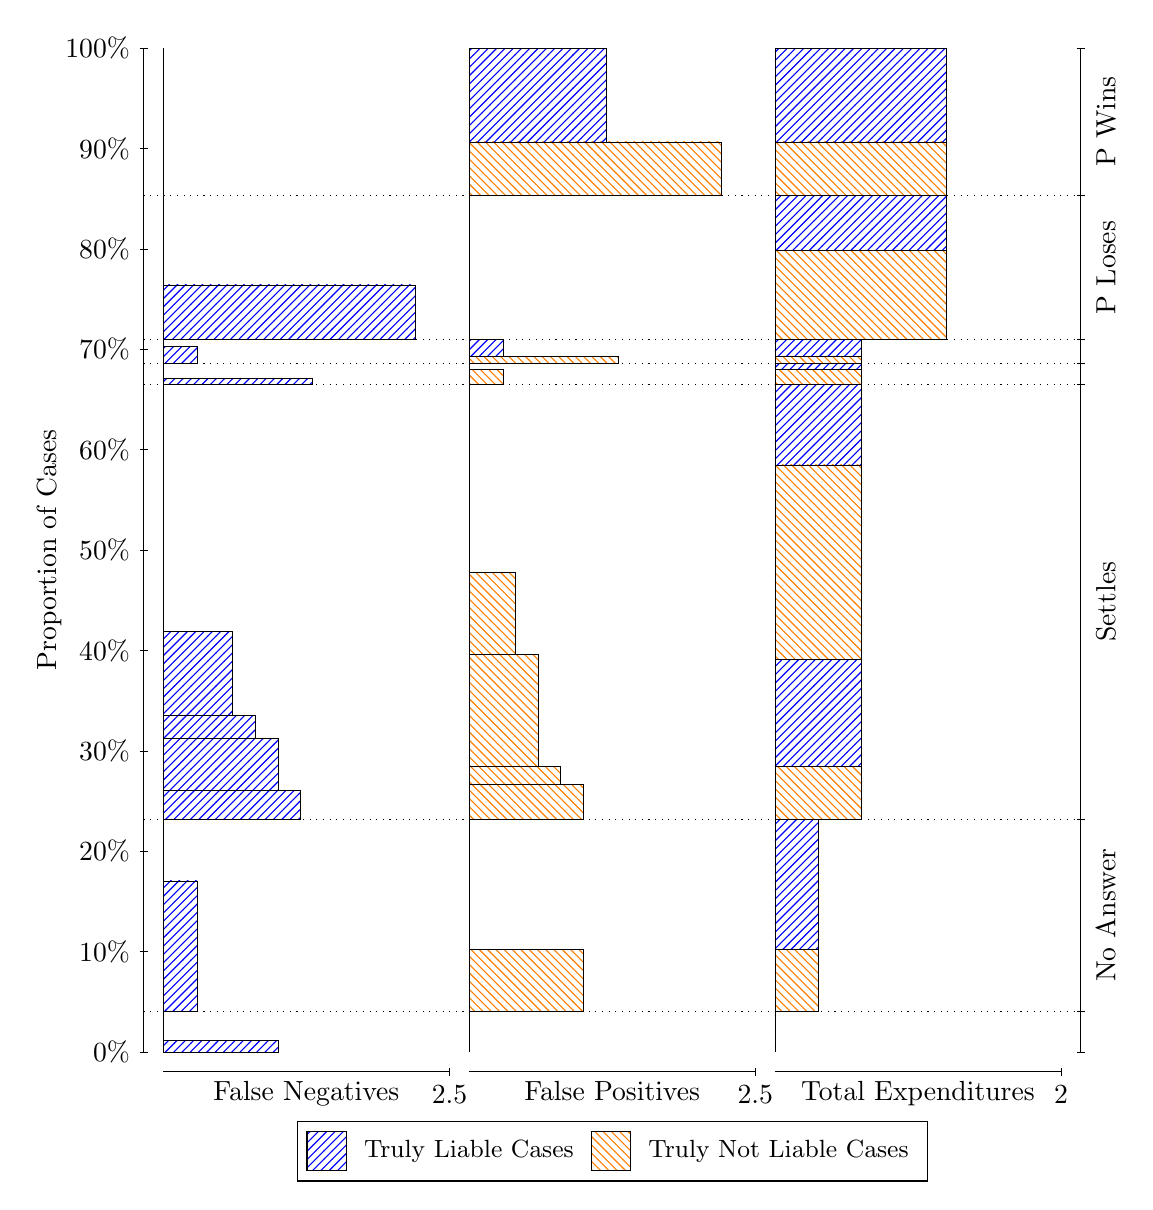
\begin{tikzpicture}
\draw[black, very thin] (1.5,1.75) -- (1.5,14.5);
\node[rotate=90, text=black, anchor=center] at (0.3, 8.125) {Proportion of Cases};
\draw[black, very thin] (1.45,1.75) -- (1.55,1.75);
\node[text=black, anchor=east] at (1.45, 1.75) {0\%};
\draw[black, very thin] (1.45,3.025) -- (1.55,3.025);
\node[text=black, anchor=east] at (1.45, 3.025) {10\%};
\draw[black, very thin] (1.45,4.3) -- (1.55,4.3);
\node[text=black, anchor=east] at (1.45, 4.3) {20\%};
\draw[black, very thin] (1.45,5.575) -- (1.55,5.575);
\node[text=black, anchor=east] at (1.45, 5.575) {30\%};
\draw[black, very thin] (1.45,6.85) -- (1.55,6.85);
\node[text=black, anchor=east] at (1.45, 6.85) {40\%};
\draw[black, very thin] (1.45,8.125) -- (1.55,8.125);
\node[text=black, anchor=east] at (1.45, 8.125) {50\%};
\draw[black, very thin] (1.45,9.4) -- (1.55,9.4);
\node[text=black, anchor=east] at (1.45, 9.4) {60\%};
\draw[black, very thin] (1.45,10.675) -- (1.55,10.675);
\node[text=black, anchor=east] at (1.45, 10.675) {70\%};
\draw[black, very thin] (1.45,11.95) -- (1.55,11.95);
\node[text=black, anchor=east] at (1.45, 11.95) {80\%};
\draw[black, very thin] (1.45,13.225) -- (1.55,13.225);
\node[text=black, anchor=east] at (1.45, 13.225) {90\%};
\draw[black, very thin] (1.45,14.5) -- (1.55,14.5);
\node[text=black, anchor=east] at (1.45, 14.5) {100\%};

\draw[black, very thin] (13.4,1.75) -- (13.4,14.5);
\draw[black, very thin] (13.35,1.75) -- (13.45,1.75);
\node[anchor=west] at (13.35, 1.75) {};
\draw[black, very thin] (13.35,2.2634) -- (13.45,2.2634);
\node[anchor=west] at (13.35, 2.2634) {};
\draw[black, very thin] (13.35,4.708) -- (13.45,4.708);
\node[anchor=west] at (13.35, 4.708) {};
\draw[black, very thin] (13.35,10.227) -- (13.45,10.227);
\node[anchor=west] at (13.35, 10.227) {};
\draw[black, very thin] (13.35,10.497) -- (13.45,10.497);
\node[anchor=west] at (13.35, 10.497) {};
\draw[black, very thin] (13.35,10.797) -- (13.45,10.797);
\node[anchor=west] at (13.35, 10.797) {};
\draw[black, very thin] (13.35,12.63) -- (13.45,12.63);
\node[anchor=west] at (13.35, 12.63) {};
\draw[black, very thin] (13.35,14.5) -- (13.45,14.5);
\node[anchor=west] at (13.35, 14.5) {};

\draw[black, very thin, pattern color=blue, pattern=north east lines] (1.75,1.75) rectangle (3.2033,1.8979);
\draw[black, very thin, pattern color=orange, pattern=north west lines] (1.75,1.8979) rectangle (1.75,2.2634);
\draw[black, very thin, pattern color=blue, pattern=north east lines] (1.75,2.2634) rectangle (2.186,3.9224);
\draw[black, very thin, pattern color=orange, pattern=north west lines] (1.75,3.9224) rectangle (1.75,4.708);
\draw[black, very thin, pattern color=blue, pattern=north east lines] (1.75,4.708) rectangle (3.494,5.0735);
\draw[black, very thin, pattern color=blue, pattern=north east lines] (1.75,5.0735) rectangle (3.2033,5.7288);
\draw[black, very thin, pattern color=blue, pattern=north east lines] (1.75,5.7288) rectangle (2.9127,6.0265);
\draw[black, very thin, pattern color=blue, pattern=north east lines] (1.75,6.0265) rectangle (2.622,7.0962);
\draw[black, very thin, pattern color=orange, pattern=north west lines] (1.75,7.0962) rectangle (1.75,10.227);
\draw[black, very thin, pattern color=blue, pattern=north east lines] (1.75,10.227) rectangle (3.6393,10.302);
\draw[black, very thin, pattern color=orange, pattern=north west lines] (1.75,10.302) rectangle (1.75,10.497);
\draw[black, very thin, pattern color=blue, pattern=north east lines] (1.75,10.497) rectangle (2.186,10.713);
\draw[black, very thin, pattern color=orange, pattern=north west lines] (1.75,10.713) rectangle (1.75,10.797);
\draw[black, very thin, pattern color=blue, pattern=north east lines] (1.75,10.797) rectangle (4.9473,11.493);
\draw[black, very thin, pattern color=orange, pattern=north west lines] (1.75,11.493) rectangle (1.75,12.63);
\draw[black, very thin, pattern color=orange, pattern=north west lines] (1.75,12.63) rectangle (1.75,13.307);
\draw[black, very thin, pattern color=blue, pattern=north east lines] (1.75,13.307) rectangle (1.75,14.5);
\draw[black, very thin, pattern color=orange, pattern=north west lines] (5.6333,1.75) rectangle (5.6333,2.1155);
\draw[black, very thin, pattern color=blue, pattern=north east lines] (5.6333,2.1155) rectangle (5.6333,2.2634);
\draw[black, very thin, pattern color=orange, pattern=north west lines] (5.6333,2.2634) rectangle (7.0867,3.049);
\draw[black, very thin, pattern color=blue, pattern=north east lines] (5.6333,3.049) rectangle (5.6333,4.708);
\draw[black, very thin, pattern color=orange, pattern=north west lines] (5.6333,4.708) rectangle (7.0867,5.1467);
\draw[black, very thin, pattern color=orange, pattern=north west lines] (5.6333,5.1467) rectangle (6.796,5.3732);
\draw[black, very thin, pattern color=orange, pattern=north west lines] (5.6333,5.3732) rectangle (6.5053,6.802);
\draw[black, very thin, pattern color=orange, pattern=north west lines] (5.6333,6.802) rectangle (6.2147,7.8386);
\draw[black, very thin, pattern color=blue, pattern=north east lines] (5.6333,7.8386) rectangle (5.6333,10.227);
\draw[black, very thin, pattern color=orange, pattern=north west lines] (5.6333,10.227) rectangle (6.0693,10.422);
\draw[black, very thin, pattern color=blue, pattern=north east lines] (5.6333,10.422) rectangle (5.6333,10.497);
\draw[black, very thin, pattern color=orange, pattern=north west lines] (5.6333,10.497) rectangle (7.5227,10.581);
\draw[black, very thin, pattern color=blue, pattern=north east lines] (5.6333,10.581) rectangle (6.0693,10.797);
\draw[black, very thin, pattern color=orange, pattern=north west lines] (5.6333,10.797) rectangle (5.6333,11.933);
\draw[black, very thin, pattern color=blue, pattern=north east lines] (5.6333,11.933) rectangle (5.6333,12.63);
\draw[black, very thin, pattern color=orange, pattern=north west lines] (5.6333,12.63) rectangle (8.8307,13.307);
\draw[black, very thin, pattern color=blue, pattern=north east lines] (5.6333,13.307) rectangle (7.3773,14.5);
\draw[black, very thin, pattern color=orange, pattern=north west lines] (9.5167,1.75) rectangle (9.5167,2.1155);
\draw[black, very thin, pattern color=blue, pattern=north east lines] (9.5167,2.1155) rectangle (9.5167,2.2634);
\draw[black, very thin, pattern color=orange, pattern=north west lines] (9.5167,2.2634) rectangle (10.062,3.049);
\draw[black, very thin, pattern color=blue, pattern=north east lines] (9.5167,3.049) rectangle (10.062,4.708);
\draw[black, very thin, pattern color=orange, pattern=north west lines] (9.5167,4.708) rectangle (10.607,5.3732);
\draw[black, very thin, pattern color=blue, pattern=north east lines] (9.5167,5.3732) rectangle (10.607,6.7405);
\draw[black, very thin, pattern color=orange, pattern=north west lines] (9.5167,6.7405) rectangle (10.607,9.2059);
\draw[black, very thin, pattern color=blue, pattern=north east lines] (9.5167,9.2059) rectangle (10.607,10.227);
\draw[black, very thin, pattern color=orange, pattern=north west lines] (9.5167,10.227) rectangle (10.607,10.422);
\draw[black, very thin, pattern color=blue, pattern=north east lines] (9.5167,10.422) rectangle (10.607,10.497);
\draw[black, very thin, pattern color=orange, pattern=north west lines] (9.5167,10.497) rectangle (10.607,10.581);
\draw[black, very thin, pattern color=blue, pattern=north east lines] (9.5167,10.581) rectangle (10.607,10.797);
\draw[black, very thin, pattern color=orange, pattern=north west lines] (9.5167,10.797) rectangle (11.697,11.933);
\draw[black, very thin, pattern color=blue, pattern=north east lines] (9.5167,11.933) rectangle (11.697,12.63);
\draw[black, very thin, pattern color=orange, pattern=north west lines] (9.5167,12.63) rectangle (11.697,13.307);
\draw[black, very thin, pattern color=blue, pattern=north east lines] (9.5167,13.307) rectangle (11.697,14.5);
\draw[black, dotted] (1.5,2.2634) -- (13.4,2.2634);
\draw[black, dotted] (1.5,4.708) -- (13.4,4.708);
\draw[black, dotted] (1.5,10.227) -- (13.4,10.227);
\draw[black, dotted] (1.5,10.497) -- (13.4,10.497);
\draw[black, dotted] (1.5,10.797) -- (13.4,10.797);
\draw[black, dotted] (1.5,12.63) -- (13.4,12.63);
\draw[black, very thin] (1.75,1.5) -- (5.3833,1.5);
\node[text=black, anchor=north] at (3.5667, 1.5) {False Negatives};
\draw[black, very thin] (5.3833,1.45) -- (5.3833,1.55);
\node[text=black, anchor=north] at (5.3833, 1.45) {2.5};

\draw[black, very thin] (5.6333,1.5) -- (9.2667,1.5);
\node[text=black, anchor=north] at (7.45, 1.5) {False Positives};
\draw[black, very thin] (9.2667,1.45) -- (9.2667,1.55);
\node[text=black, anchor=north] at (9.2667, 1.45) {2.5};

\draw[black, very thin] (9.5167,1.5) -- (13.15,1.5);
\node[text=black, anchor=north] at (11.333, 1.5) {Total Expenditures};
\draw[black, very thin] (13.15,1.45) -- (13.15,1.55);
\node[text=black, anchor=north] at (13.15, 1.45) {2};


\node[text=black, centered, rotate=90] at (13.72, 3.4857) {No Answer};
\node[text=black, centered, rotate=90] at (13.72, 7.4674) {Settles};


\node[text=black, centered, rotate=90] at (13.72, 11.713) {P Loses};
\node[text=black, centered, rotate=90] at (13.72, 13.565) {P Wins};

\draw (7.449999999999999,1.5) node[draw=none] (baseCoordinate) {};
\begin{scope}[align=center]
        \matrix[scale=0.5, draw=black, below=0.5cm of baseCoordinate, nodes={draw}, column sep=0.1cm]{
            \node[rectangle, draw, minimum width=0.5cm, minimum height=0.5cm, pattern color=blue, pattern=north east lines] {}; &
            \node[draw=none, font=\small, text=black] (B) {Truly Liable Cases}; &
            \node[rectangle, draw, minimum width=0.5cm, minimum height=0.5cm, pattern color=orange, pattern=north west lines] {}; &
            \node[draw=none, font=\small, text=black] (B) {Truly Not Liable Cases}; \\
            };
\end{scope}

\end{tikzpicture}
\end{document}